\listfiles
\documentclass{article}

\usepackage{tikz}
\usetikzlibrary{math}

\begin{document}

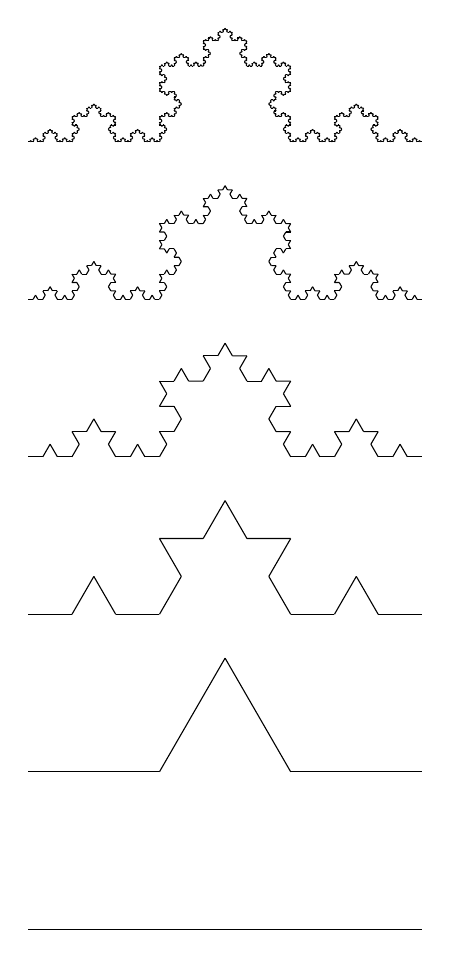
\begin{tikzpicture}
    \tikzmath{
        function snowline (\xStart, \yStart, \xEnd, \yEnd, \depth) {
            \xU = \xEnd - \xStart;
            \yU = \yEnd - \yStart;
            \xV = \yStart - \yEnd;
            \yV = \xEnd - \xStart;
            \xP = \xStart + \xU / 3;
            \yP = \yStart + \yU / 3;
            \xQ = \xStart + \xU / 2 + sqrt(3) / 6 * (\xV);
            \yQ = \yStart + \yU / 2 + sqrt(3) / 6 * (\yV);
            \xR = \xStart + 2/3 * \xU;
            \yR = \yStart + 2/3 * \yU;
%
            if (\depth == 0) then {
                {\draw (\xStart,\yStart) -- (\xEnd,\yEnd); };
            } else {
                \nd = \depth - 1;
                snowline(\xStart,\yStart,\xP,\yP,\nd);
                snowline(\xP,\yP,\xQ,\yQ,\nd);
                snowline(\xQ,\yQ,\xR,\yR,\nd);
                snowline(\xR,\yR,\xEnd,\yEnd,\nd);
            };
        };
%
%
        for \d in {0,...,5}{
            snowline(0, 2*\d, 5, 2*\d, \d);
        };
    }
\end{tikzpicture}

\end{document}
